\documentclass[lang=english,inputenc=utf8,fontsize=10pt]{ldvarticle}
\usepackage{graphicx}
\usepackage{setspace}
\usepackage{csquotes}
\usepackage[ddmmyyyy]{datetime}
\usepackage{amsmath}
\usepackage{hyperref}

\usepackage{parskip}
\usepackage{subfigure}
\usepackage{ifthen}
\usepackage{comment}
\usepackage{color}
\usepackage{colortbl}
\usepackage{soul}
\usepackage{tikz}
\usetikzlibrary{shapes,arrows}
\usepackage{tabularx}

\definecolor{lightgray}{rgb}{0.75,0.75,0.75}



\title{\# Stay at home --- Are Germany's greenhouse gas emissions increasing or decreasing}
\subtitle{Proposal of Group 5}
\author{Robert Annuth\\
03723414
\and
Laura Pilger\\
03735972
\and
Mohamed Badawy\\
03722512
\and
Natalia Voronova\\
03691009
\and
Utku Ayvaz\\
03690266
\and
Noah Binh Nguyen\\
03683505
\and
Mariem Nouicer\\
03687720
\and
fell\\
free
\and
adding\\
your
\and
names\\
here
}

\date{\today}

\begin{document}


\maketitle
\thispagestyle{empty}

\hrule

\section*{Motivation}


Besides the current Covid-19 issue the population of the whole world is facing the climate change. Almost all human activities cause or lead to greenhouse gas emissions, which drive up the temperature. Extreme weather and melting polar ice are other possible effects. Consequently it is highly relevant to identify economic sectors and human behavior with the potential to decrease emissions.\\

Current research regarding this topic is mostly based on mathematical models and can not be verified by actual data. Due to the restrictions of the Covid-19 crisis the human behavior has transformed, which creates ground truth data and the possibility to conclude how to decease greenhouse gas emissions based on the restrictions and human behavior during the crisis.\\

\vspace*{1cm}
\hrule

\newpage

\section{Project Description}
On the one hand economic sectors can be analysed and potential factors derived, which lead to decreasing emissions. On the other hand the general question \enquote{What can we do?}, which refers to the actions every human can take, can be answered based on actual data.\\
Our group wants to focus on Germany. However, it is possible to answer the question for different countries or areas.\\

\section*{Research Question}
This research analyses which human behavior, during the Covid-19 crisis, is increasing or decrasing greenhouse gas emissions. The increase or decrease is measuread in respect to the time before the cirsis.\\

\section*{Goals}
Our goal is to find human behavior, decreasing the total greenhouse gas emissions. We think that some of our current behavior is stronly influencing the total emissions. Hence, it is interesting to find out how each economic sector is influenced. Besides we are curious to find out if there is human behavior which is sinificantly decreasing the total emissions and could be maintained beyond the crisis to archive the climate agreement.\\

\section*{Approaches}
In our group were many concerns, if we will find enough information to verify the predictions of our model. So we spend much time to find possible data sources to answer the research question. The task for this milestone is not to find data source, so we decided to group our current sources into general topics. Each of these topice could be an approach or predictor to answer the research question.\\

\begin{itemize}
    \item The German \enquote{Umweltbundesamt} is providing actual CO2 data
    \item Real time monitoring of greenhouse gases with satellite pictures
    \item Information from economic sectors can be used as additional predictor --- for example the electricity sector
    \item The consumption of resources (oil, coal,...)
    \item Stock market information
\end{itemize}

\newpage

\section{Work packages}
\label{workp}
Our group found a detailed explanation how to structure larger machine learning project and we agreed to follow this guide. (\href{https://www.jeremyjordan.me/ml-projects-guide/}{link}) \\
Nevertheless, the guide is mostly concluding what we discussed inside the breakout rooms during the second lecture.\\
\begin{itemize}
    \item \textbf{Planning and project setup}
    \begin{itemize}
        \item Define the task and scope out requirements
        \item Determine project feasibility
        \item Discuss general model tradeoffs (accuracy vs speed)
        \item Set up project codebase
    \end{itemize}
    \item \textbf{Data collection and labeling}
    \begin{itemize}
        \item Define ground truth (create labeling documentation)
        \item Build data ingestion pipeline
        \item Validate quality of data
        \item Revisit Step 1 and ensure data is sufficient for the task
    \end{itemize}
    \item \textbf{Model exploration}
    \begin{itemize}
        \item Establish baselines for model performance
        \item Start with a simple model using initial data pipeline
        \item Overfit simple model to training data
        \item Stay nimble and try many parallel (isolated) ideas during early stages
        \item Find SoTA model for your problem domain (if available) and reproduce results, then apply to your dataset as a second baseline
        \item Revisit Step 1 and ensure feasibility
        \item Revisit Step 2 and ensure data quality is sufficient
    \end{itemize}
    \item \textbf{Model refinement}
    \begin{itemize}
        \item Perform model-specific optimizations (ie. hyperparameter tuning)
        \item Iteratively debug model as complexity is added
        \item Perform error analysis to uncover common failure modes
        \item Revisit Step 2 for targeted data collection of observed failures
    \end{itemize}
    \item \textbf{Testing and evaluation}
    \begin{itemize}
        \item Evaluate model on test distribution; understand differences between train and test set distributions (how is “data in the wild” different than what you trained on)
        \item Revisit model evaluation metric; ensure that this metric drives desirable downstream user behavior
        \item Write tests for:
        \begin{itemize}
            \item Input data pipeline
            \item Model inference functionality
            \item Model inference performance on validation data
            \item Explicit scenarios expected in production (model is evaluated on a curated set of observations)
        \end{itemize}
    \end{itemize}
\end{itemize}

\section{Workload distribution}
As we are at the beginning of the project phase we agreed to define work packages but wait with the assignmend. However, we decided to assign specialists to certain tasks (table \ref{tab:special}). The specialists have experience to accomplish their task and therefore they are responsible to keep track of the process and improve the work flow.\\


\begin{table}[ht]
\begin{tabular}{l|l|l}
Task                      & Responsible Person  & Description                             \\ \hline
Data Engineer             & Samra               & Collecting Data, Quality, Preprocessing \\
Machine Learning Engineer & Mohamed, Utku, Noah & Model creation                          \\
Software Engineer         & Mariem              & Front End                               \\
Project Manager           & Zubair              & Planning, Documentation                 \\
Submissions               & Laura, Robert       & Report                                  \\
Video                     & Natalia             &                                        
\end{tabular}
\caption{Project tasks assigned to specialists}
\label{tab:special}
\end{table}
During the project phase we want to have a long planning meeting at the beginning of each milestone to divide the tasks of the milestone using the work packages mentioned in section \ref{workp} and assign people to them.\\

\newpage

\section{Risk Analysis}
Our group tried to identify possible risks during the project phase. The following list contains the results of a short brainstorming.\\

\begin{itemize}
    \item Quality of the data
    \item Not enough data
    \item No existing data for performance measurement - No ground truth
    \item We are discussing a complex issue, obtaining clear results can be difficult
    \item No program for video editing
    \item Not enough computing power to train the models
    \item Version control (updates of packages)
    \item Organisational issues (no personal meetings, big group, conflict potentials)
    \item Other lectures (overlapping deadlines)
    \item Research question is too complex
\end{itemize}

After some discussion we agreed, that we are facing two risk. One is not to find enough data, which would make it impossible to make good predictions. The other issue is that we could be unable to conclude which human behavior is causing decreased or increased emissions, because the correlation is too complex.\\
The other issues result in additional workload but do not jeopardise the project. However, with the possible data sources mentioned earlier we are confident, that we are well prepared for the project phase.\\



\section{Time Table}

We decided to organise our project using a Gantt chart. Where we are including all milestones and additional tasks required to fulfill each milestone. Fig. \ref{fig:projplan} shows a short overview of the current plan. The last milestone is collapsed to show is clearly.\\
When Milestone I is reached, we plan our steps for Milestone II. The reason we are planing each Milestone sperately is because we think this research project is rather dynamic. The topic is new and the goal of the lecture is to apply machine leanring in a large group. This means at the moment we do not have enough knowledge to plan the whole project phase. We want to be able to learn of the failures from the previous milestone. Hence, the time table is updated for each milestone.\\
Besides the dynamic project planning method is mostly favored for research projects, because it is diffucult to plan new terretory.\\


\begin{figure}[ht]
\rotatebox{90}{%
\begin{minipage}{1.5\textwidth}
\centering
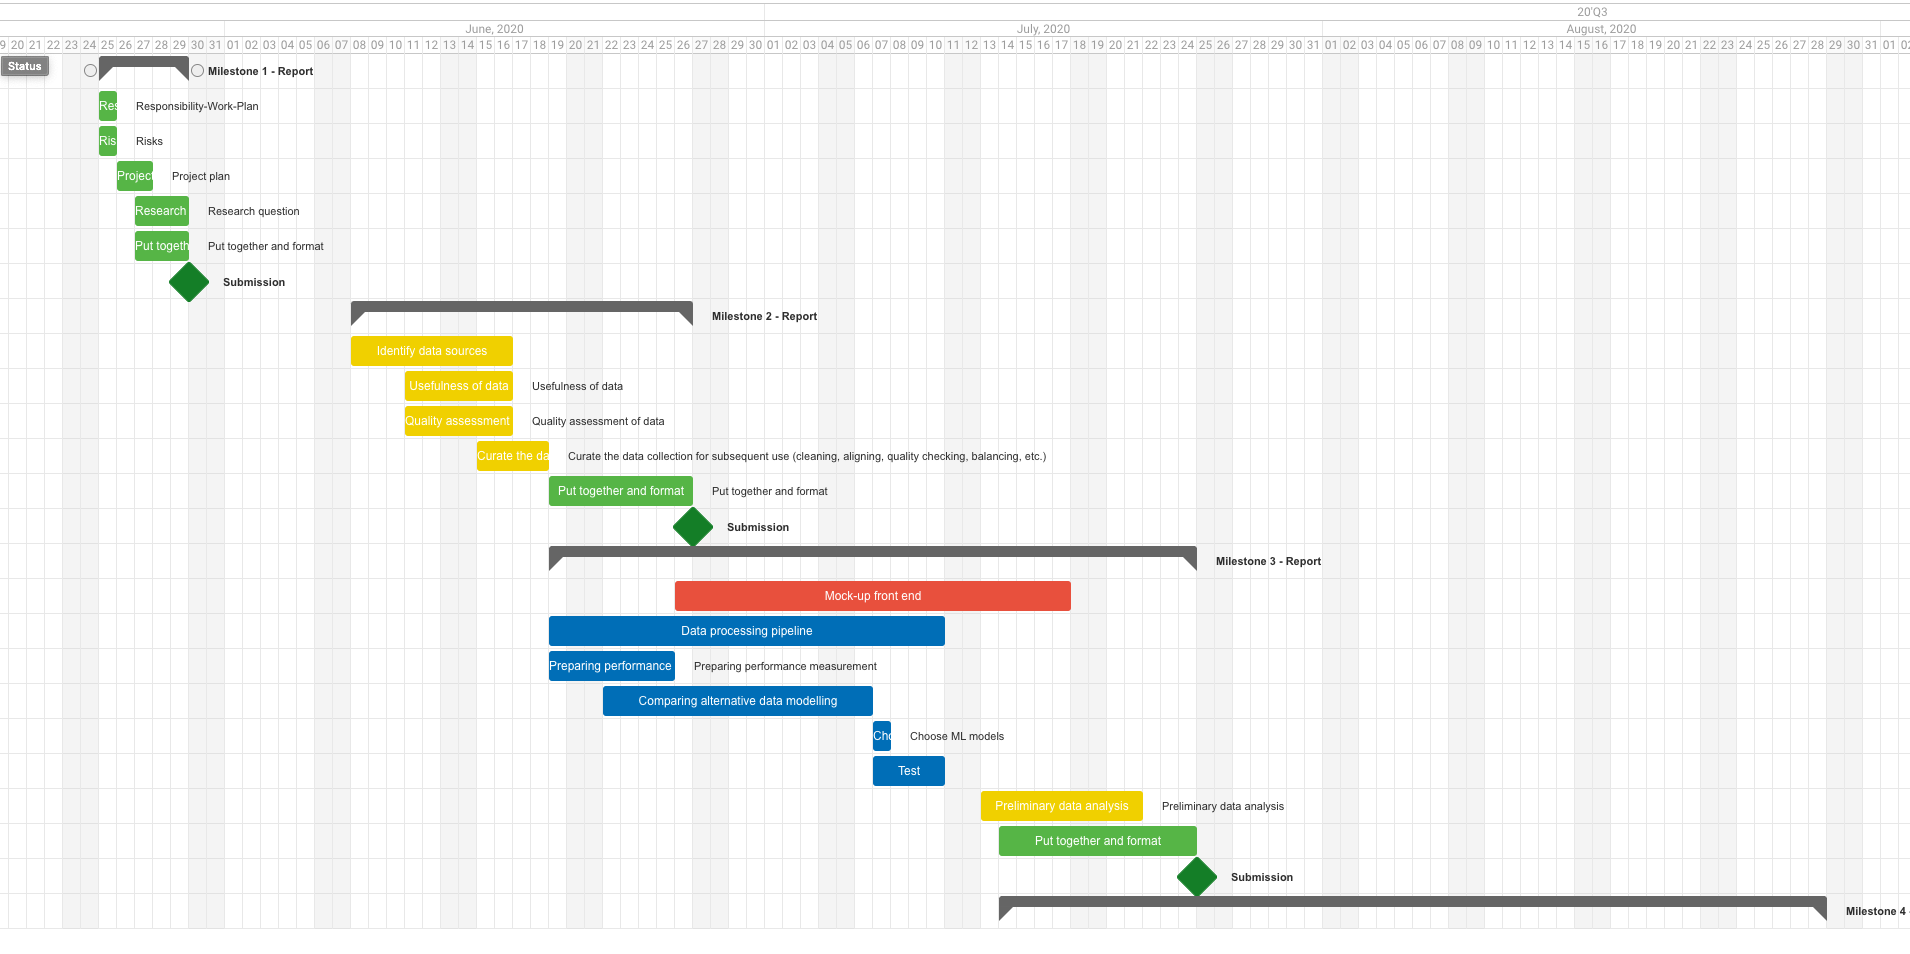
\includegraphics[width=0.99\textwidth]{fig/gantt}
    \caption{Gantt Project Plan (24.05.2020)}%
    \label{fig:projplan}
\end{minipage}
}
\end{figure}

\end{document}
